Um die gestellte Moduldatenbank in unseren Entwurf zu integrieren, haben wir diese um \textit{Fields} (Bereiche) und \textit{Rule-Groups} erweitert.

\textit{Fields} modellieren Bereiche eines Studiengangs. Zu jedem Bereich gehört eine Mindestanzahl an ECTS, die ihn ihm belegt werden müssen. Ist das Attribut \textit{choosable} gesetzt, so verfügt ein Bereich auch über Vertiefungsfächer. Damit kann der Benutzer bei der Generierung in jedem auswählbaren Bereich ein Vertiefungsfach angeben, aus welchem der Generierer bevorzugt Module wählen soll. Diese Änderung sorgt unter anderem dafür, dass die nötigen 180~ECTS für den Bachelor nicht hartkodiert werden müssen, sondern aus der Summe der ECTS der zu einem Studiengang gehörigen Bereiche berechnet werden können.

\textit{Rule-Groups} beschreiben Gruppen von Modulen, die bezüglich Modulanzahl beschränkt sind. Das heißt, dass innerhalb einer Gruppe eine Mindest- und eine Maximalanzahl an Modulen vorgeschrieben sind, um ein Studienfach erfolgreich abschließen zu können. Dies stellt zum Beispiel sicher, dass mindestens zwei Stammmodule sowie ein Proseminar belegt werden.

Diese Änderungen ermöglichen eine stärkere Abstraktion der Bedingungen eines Studiengangs, was die Modellierung von unterschiedlichen Studiengängen vereinfacht.

\begin{figure}
	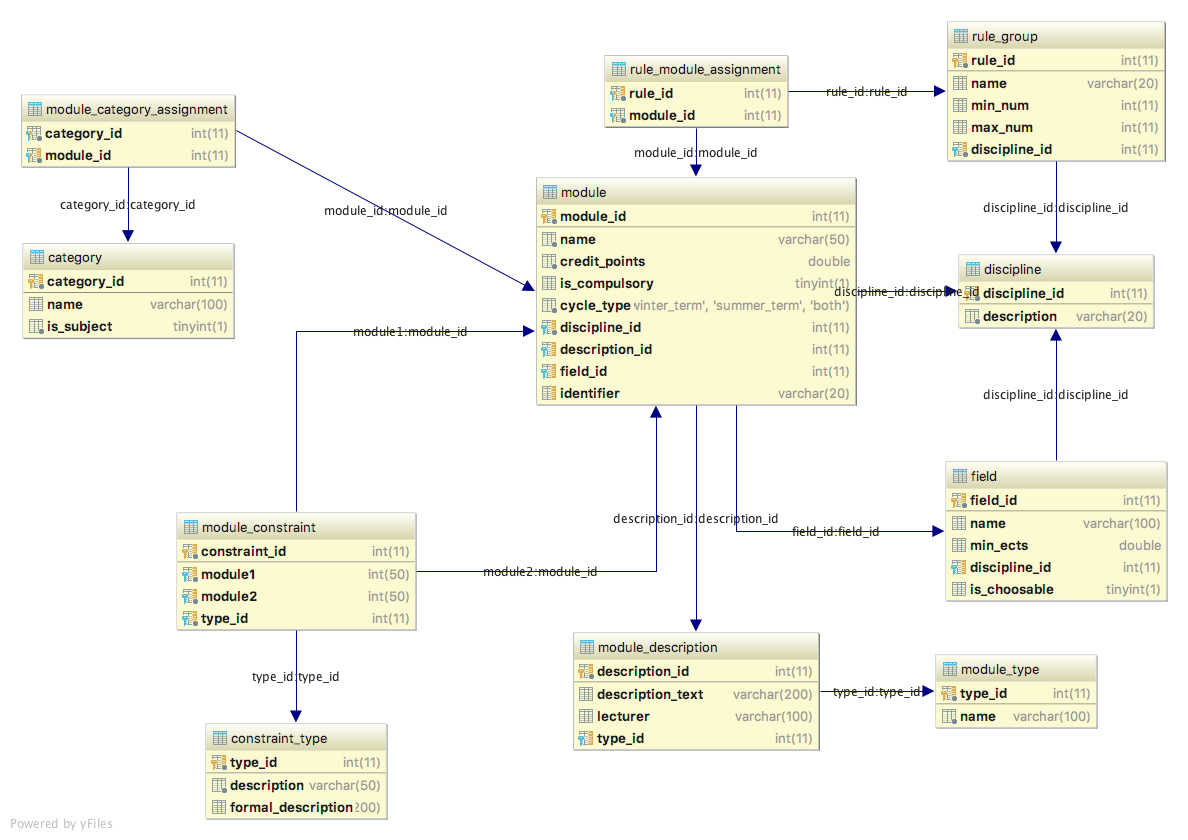
\includegraphics[width = \textwidth]{diagrams/module_diagram.png}
	\caption{Übersicht über die Struktur der Moduldatenbank}
\end{figure}